\chapter{Experiments}
\label{ch:exp}

\section{Datasets}

We adapt Breakfast~\cite{kuehne2014language}, CrossTask~\cite{zhukov2019crosstask}, and YouTube Instructional~\cite{alayrac2016unsupervised}  datasets to the incremental learning setup. Note other TAS datasets such as GTEA~
\cite{fathi2011learning} and 50Salads~\cite{stein2013combining} are unsuitable because most of their videos share a common set of actions, making it challenging to implement a meaningful number of incremental tasks without a significant action overlap.

% Please add the following required packages to your document preamble:
% \usepackage{multirow}
% \usepackage[table,xcdraw]{xcolor}
% Beamer presentation requires \usepackage{colortbl} instead of \usepackage[table,xcdraw]{xcolor}
\begin{table}[!h]
\begin{tabular}{lccccc}
\toprule
Dataset    & \# Videos & Duration & \# Activities & \# Actions & Domain \\ \cmidrule(lr){1-1} \cmidrule(lr){2-6}
Breakfast~\cite{kuehne2014language}  & 1712     & 77h      &  10          &  48       & Cooking \\ 
CrossTask~\cite{zhukov2019crosstask}* & 2140     & 170h     &  14          &  112      & Mixed \\ 
YTI~\cite{alayrac2016unsupervised}       & 150      & 7h       &  5           &  46       & Mixed \\ \bottomrule
\end{tabular}
\footnotesize{*CrossTask processed as described in~\cref{sub:crosstak}.}
\caption{
    Summary of iTAS Datasets. 
}
\label{tab:dataset_stats}
\end{table}

\subsection{Breakfast}

Breakfast~\cite{kuehne2014language} dataset is composed of 1,712 cooking videos, totalling to approximately 77 hours of footage. It consists of 52 participants performing everyday breakfast preparation tasks. The videos were recorded in 18 different kitchen settings from multiple camera views. Participants were completely undirected. Thus, the dataset contains significant variability in both action choice and action sequence order, making it a challenging benchmark in TAS.

There are 10 cooking activities and a total of 48 action classes. Each activity features 5 to 14 actions and comprises around $150$ videos for training and $20\!-\!30$ for testing. Each video contains 6.8 action segments on average. We use the I3D~\cite{carreira2017quo} feature representations and evaluate with the standard splits.

\subsection{CrossTask}
\label{sub:crosstak}

CrossTask~\cite{zhukov2019crosstask} is a large dataset  composed of 4,713 videos demonstrating 83 activities. Of these activities, only the 18 activities categorized as \emph{primary} are fully annotated with temporal locations of each action segment, while the remaining 65 activities are not. We adapt the 18 primary activities into incremental temporal action segmentation.

Within the 18 primary activities, some activities have significant overlap with others. For example, $80\%$ of the actions in \emph{``make irish coffee''} is shared with activities like \emph{``make latte''} and \emph{``make jello shots''}. We manually filter out activities with a large overlap to maintain a level of distinctiveness between tasks. After filtering, the CrossTask dataset we use is composed of 2,140 videos totalling to around 170 hours of footage. There are 14 activities and 112 actions. Each activity contains 6 to 12 actions. Each video has 14.6 action segments on average.

We use 80\% of the videos in each activity for training and reserve the remaining for evaluation. We use the feature representation designed by the authors of the dataset, which is concatenated from the RGB I3D~\cite{carreira2017quo}, ResNet-152~\cite{he2016resnet}, and audio~\cite{hershey2017cnnaudio} features extracted from one second temporal windows.

\subsection{YouTube Instructional}

YouTube Instructional (YTI)~\cite{alayrac2016unsupervised}  dataset is composed of 150 narrated instructional videos collected from YouTube, totalling to around 7 hours of footage. The dataset comprises of 5 activities with 30 video samples for each activity. There are a total of 46 actions with each activity featuring 6 to 13 actions. Each video sample contains 17.2 action segments on average.

Similar to CrossTask, we use 80\% of the videos in each activity for training and reserve the remaining for evaluation. We use the same set of feature representations as~\cite{sener2018unsupervised,kukleva2019unsupervised}, which is formed by concatenating motion (bag-of-visual-word HOF~\cite{wang2013action}) and appearance (VGG-16~\cite{simonyan2015very}) features.

\subsection{Adapting for iTAS}

We partition the Breakfast, CrossTask, and YTI  datasets based on activities. Each activity is a separate task, and we train models incrementally on them. We experiment with both disjoint and blurry incremental settings on Breakfast. 

Disjoint tasks consider shared actions different, e.g., \emph{`take plate'} in \emph{``friedegg''} is a different class from \emph{`take plate'} in \emph{``sandwich''}. In the blurry setup for Breakfast, overlapping tasks are allowed, such that common actions between tasks are the assigned the same class label.

Breakfast, CrossTask, and YTI all contain background frames, which are frames that do not depict the task taking place (e.g. narration). We treat these background frames as another action class and include them during training and evaluation.

\section{Evaluation Metrics}

Temporal action segmentation is evaluated by a frame-wise accuracy (Acc), segment-wise edit score (Edit), and F1 score with varying overlap thresholds of 10\%, 25\%, and 50\%~\cite{ding_temporal_2023}. We adopt these standard measures and apply them to the incremental setup.

\subsection{Frame-wise Metrics}

Frame-wise accuracy (Acc), also known as Mean over Frames in TAS literature, is the percentage of the model's correct frame predictions, i.e.,
\begin{equation}
    \text{Acc} = \left( \frac{\text{\# of correct predictions}}{\text{\# of predictions}} \right) * 100
\end{equation}

It gives a good measure of the model's action classification capabilities. However, it fails to capture the segment quality in the model's output. Over-segmentation is a phenomenon where an action segment is fragmented into discontinuous sub-segments by erroneous frame predictions. Though a model's predictions may exhibit over-segmentation, a high Acc score can still be reported if the incorrect predictions are comparatively few and interspersed. To capture the quality of the segments in a model's output, we must also evaluate the predictions on segment-wise measures.

\subsection{Segment-wise Metrics}

The edit score~\cite{lea2016segmentscore} is a segment-wise metric based on the Levenshtein edit distance.  The edit distance $e[|X|,|Y|]$ between two action sequences $X$ and $Y$ is given by the minimum number of edit operations (i.e. insertion, deletion, replacement) required to transform one sequence to another. The $e[|X|,|Y|]$ distance is normalized to get the edit score, i.e.,
\begin{equation}
    \text{Edit} = \left( 1 - \frac{e[|X|,|Y|]}{max(|X|,|Y|)} \right) * 100
\end{equation}
The edit score is a useful metric that evaluates the model's ability to predict action sequence order without needing exact temporal alignment with the ground truth.

The F1 score or F1@$\tau$~\cite{lea2017tcn} is another segment-based metric and is built upon Intersection-over-Union (IoU) scores. A predicted action segment is considered a true positive of the ground truth segment if its IoU score exceeds $\frac{\tau}{100}$ and if their action labels match. Only the predicted segment with the highest IoU score in the span of the ground truth segment is considered a true positive, and any other predicted segments in the same span are marked as a false positives. Any missed ground truth segments are false negatives. From these results, the F1 score can be calculated as the harmonic mean of the precision and recall scores, i.e,
\begin{equation}
    \text{F1} = 2 \cdot \frac{\text{precision} * \text{recall}}{\text{precision} + \text{recall}}
\end{equation}
Compared to the edit score, the F1 score is stricter and can more heavily penalize over-segmentation errors.

\subsection{Evaluation in iTAS}

For iTAS, we denote the model's Acc on task $b'$ after being trained on the $b$-th task as $\text{Acc}_b^{b'}$, where $b'< b$. We use the last stage accuracy averaged over all tasks as the final metric to measure the overall performance, i.e., 
\begin{equation*}
    \text{Acc} = \frac {\sum_{b=1}^B \text{Acc}_B^b} {B}.
\end{equation*}
We calculate the average performance over all tasks due to the imbalance in frame numbers across each task. The final reported Edit and F1 scores are similarly defined, i.e., 
\begin{equation*}
    \text{Edit} = \frac {\sum_{b=1}^B \text{Edit}_B^b} {B},
\end{equation*}
\begin{equation*}
    \text{F1} = \frac {\sum_{b=1}^B \text{F1}_B^b} {B}.
\end{equation*}

\section{Implementation Details}

\subsection{TCA Model}

Our TCA model comprises an encoder and decoder; each implemented as a two-layer MLP with a 256-D latent space. We train TCA for 2,500 epochs with batch size 512 for Breakfast, 250 epochs with batch size 64 for YTI, and 250 epochs with batch size 32 for CrossTask. The learning rate is set to be $1e^{-3}$, $1e^{-5}$, and $1e^{-4}$, respectively.

\subsection{TAS Backbones}

We experiment with the temporal convolutional network MSTCN~\cite{farha2019ms} and the transformer-based ASFormer~\cite{yi2021asformer}
for our backbone model $\mathcal{M}$. MSTCN is trained with a learning rate of $5e^{-4}$ for 50 epochs for each task; for ASFormer, it is $1e^{-4}$ for 30 epochs. Both models are trained with the ADAM optimizer. 

\subsection{Replay Size}

For all experiments, we constrain the maximum number of videos for replay to 60, which is equally divided among the seen tasks. The value of 60 was chosen to maintain a similar exemplar-to-training ratio (1:25) per iCIFAR-100 used in~\cite{rebuffi2017icarl}.

Given that the action sequence of generated videos is sampled from past task video instances, the total number of frames generated as the replay buffer has an upper limit of $60\times\text{longest video}$. Our ablation study (see \cref{sec:abs_replay_size}) shows that the performance can be further improved with a larger buffer size. 

\section{Effectiveness}

\subsection{Baselines}

We first use a naive (\textbf{`Finetune'}) baseline that progressively finetunes with only training data in the task sequence without data replay. Additionally, we follow the boring baseline from action recognition~\cite{alssum2023just} and store a mean frame for each action segment per sequence, which we call \textbf{`Exemplar'}. Such a segment is static, as the frame-wise sample is simply replicated to inflate the segment in time and used for data replay. Finally, we consider an upper-bound (\textbf{`Original'}) data replay baseline that uses the original sequence features. 

\subsection{Results}

% Please add the following required packages to your document preamble:
% \usepackage{booktabs}
% \usepackage{multirow}
\begin{table}[!ht]
\centering
\scalebox{0.83}{
\begin{tabular}{clcccccccccc}
\toprule
\multirow{2}{*}{\# Tasks} & \multirow{2}{*}{} & \multicolumn{5}{c}{MSTCN~\cite{farha2019ms}} & \multicolumn{5}{c}{ASFormer~\cite{yi2021asformer}} \\ \cmidrule(lr){3-7} \cmidrule(lr){8-12}
 &  & Acc & Edit & \multicolumn{3}{c}{F1 @ \{10, 25, 50\}} & Acc & Edit & \multicolumn{3}{c}{F1 @ \{10, 25, 50\}} \\ \midrule
 &&\multicolumn{10}{c}{Breakfast}\\\midrule
\multirow{4}{*}{10} & Finetune & 7.4 & 7.2 & 7.5 & 7.0 & 5.4 & 9.9 & 9.8 & 10.3 & 9.4 & 7.5 \\
 & Exemplar~\cite{alssum2023just} & 16.1 & 13.3 & 13.8 & 12.5 & 9.5 & 12.4 & 11.2 & 11.7 & 10.7 & 8.5 \\

 &  \cellcolor{gray!30}Ours & \cellcolor{gray!30}\textbf{29.4} & \cellcolor{gray!30}\textbf{25.9} & \cellcolor{gray!30}\textbf{26.3} & \cellcolor{gray!30}\textbf{23.5} & \cellcolor{gray!30}\textbf{17.7} & \cellcolor{gray!30}\textbf{34.2} & \cellcolor{gray!30}\textbf{32.4} & \cellcolor{gray!30}\textbf{33.1} & \cellcolor{gray!30}\textbf{30.1} & \cellcolor{gray!30}\textbf{23.4} \\
 & \textcolor{gray}{Original} & \textcolor{gray}{43.1} & \textcolor{gray}{41.1} & \textcolor{gray}{41.2} & \textcolor{gray}{37.6} & \textcolor{gray}{29.5} & \textcolor{gray}{48.1} & \textcolor{gray}{45.2} & \textcolor{gray}{45.9} & \textcolor{gray}{42.4} & \textcolor{gray}{34.2} \\ \midrule
\multirow{4}{*}{5} & Finetune & 15.4 & 15.8 & 16.6 & 15.8 & 12.7 & 15.7 & 16.1 & 16.9 & 15.8 & 13.2 \\
 & Exemplar~\cite{alssum2023just} & 32.5 & 28.9 & 30.8 & 28.5 & 22.9 & 29.5 & 27.5 & 28.7 & 26.7 & 22.0 \\
 & \cellcolor{gray!30}Ours & \cellcolor{gray!30}\textbf{54.5} & \cellcolor{gray!30}\textbf{49.4} & \cellcolor{gray!30}\textbf{51.1} & \cellcolor{gray!30}\textbf{46.9} & \cellcolor{gray!30}\textbf{37.7} & \cellcolor{gray!30}\textbf{57.2} & \cellcolor{gray!30}\textbf{56.8} & \cellcolor{gray!30}\textbf{58.3} & \cellcolor{gray!30}\textbf{54.0} & \cellcolor{gray!30}\textbf{43.6} \\
 & \textcolor{gray}{Original} & \textcolor{gray}{60.4} & \textcolor{gray}{59.1} & \textcolor{gray}{60.3} & \textcolor{gray}{56.1} & \textcolor{gray}{46.0} & \textcolor{gray}{65.1} & \textcolor{gray}{64.2} & \textcolor{gray}{65.6} & \textcolor{gray}{61.5} & \textcolor{gray}{51.0} \\ \midrule
&&\multicolumn{10}{c}{CrossTask}\\ \midrule
\multirow{4}{*}{14}& Finetune & 5.3 & 3.8	& 3.8 & 3.4 & 2.5 & 5.3 & 4.1 & 3.9 & 3.5 & 2.5 \\
& Exemplar~\cite{alssum2023just} & 9.8	& 6.7 & 6.5 & 5.5 & 3.6 & 12.2 & 8.5 & 8.6 & 7.4 & 5.0 \\
& \cellcolor{gray!30}Ours & \cellcolor{gray!30}\textbf{35.4} & \cellcolor{gray!30}\textbf{22.9} & \cellcolor{gray!30}\textbf{22.7} & \cellcolor{gray!30}\textbf{19.4} & \cellcolor{gray!30}\textbf{12.4} & \cellcolor{gray!30}\textbf{46.5} & \cellcolor{gray!30}\textbf{32.2} & \cellcolor{gray!30}\textbf{31.3} & \cellcolor{gray!30}\textbf{27.3} & \cellcolor{gray!30}\textbf{18.0} \\
&\textcolor{gray}{Original} & \textcolor{gray}{40.8} & \textcolor{gray}{26.9} & \textcolor{gray}{26.6} & \textcolor{gray}{23.4} & \textcolor{gray}{15.7} & \textcolor{gray}{48.5} & \textcolor{gray}{30.5} & \textcolor{gray}{31.2} & \textcolor{gray}{27.5} & \textcolor{gray}{18.3} \\ \midrule
&&\multicolumn{10}{c}{YouTube Instructional}\\ \midrule
\multirow{4}{*}{5}& Finetune & 13.6 & 2.8 & 3.6 & 2.7 & 0.6 & 13.9 & 11.5 & 11.1 & 9.8 & 6.3 \\
& Exemplar~\cite{alssum2023just} & \textbf{30.8} & 19.7 & 19.8 & 16.0 & 9.3 & 22.1 & 18.9 & 17.7 & 15.3 & 10.0 \\
& \cellcolor{gray!30}Ours & \cellcolor{gray!30}30.2 & \cellcolor{gray!30}\textbf{25.0} & \cellcolor{gray!30}\textbf{21.9}& \cellcolor{gray!30}\textbf{18.5} & \cellcolor{gray!30}\textbf{11.1} & \cellcolor{gray!30}\textbf{25.2} & \cellcolor{gray!30}\textbf{20.9} & \cellcolor{gray!30}\textbf{20.1} & \cellcolor{gray!30}\textbf{17.5} & \cellcolor{gray!30}\textbf{11.4} \\
&\textcolor{gray}{Original} & \textcolor{gray}{55.9} & \textcolor{gray}{39.4} & \textcolor{gray}{38.1} & \textcolor{gray}{32.2} & \textcolor{gray}{19.1} & \textcolor{gray}{59.2} & \textcolor{gray}{51.1} & \textcolor{gray}{45.4} & \textcolor{gray}{39.1} & \textcolor{gray}{25.5} \\ \bottomrule
\end{tabular}}
\caption{Performance comparison on Breakfast, CrossTask, and YouTube Instructional.% Our approach consistently surpasses the baselines, with both MSTCN and ASFormer backbones. %(Results are averaged over five random seeds, refer to Supplementary Materials for variations.)}%~\AY{take-away statement on performance.} ~\AY{ref supplementary for var over runs.}
}
\label{tab:all}
\end{table}

We compare the performances on three datasets in~\cref{tab:all}. We adopt the approach of prior incremental learning studies by initializing the task sequence with multiple random seeds. We utilized five specific random seeds throughout our experiments: $\{42, 123, 1000, 1993, 2023\}$. The performance results presented reflect the mean across multiple splits and seeds.

Finetune achieves the lowest performance as it simply concentrates on learning new concepts without revisiting previous tasks. In the 10-task setup on Breakfast, static segments with stored exemplar features mitigate forgetting, gaining an accuracy increase from 7.4\% to 16.1\% with MSTCN. Our approach achieves a more substantial boost, reaching 29.4\%. The improvement is consistent across both backbones. Despite this improvement, there remains a 13.1\% gap compared to using original features from previous tasks.

There are similar performance differences across the approaches in the 5-task incremental Breakfast setup. The 5-task incremental setup combines every two activities as a single task and has fewer training steps, improving performance across all approaches. This suggests that the challenge of learning increases with the number of tasks, leading to increased forgetting by the model. 

For CrossTask, our approach likewise attains impressive performance gains in all metrics compared baselines on both backbones. Accuracy jumps from the Exemplar baseline's 9.82\% to 35.41\% with MSTCN and from 12.22\% to 46.54\% with ASFormer. The edit and F1 scores also show similar improvements.

The performance gains for the YTI dataset is less significant compared to either Breakfast or CrossTask; both the Exemplar~\cite{alssum2023just} and our method achieve very similar performances. We hypothesize that this phenomenon results from the overall reduced segment diversity in the YTI dataset due to its comparatively smaller size. Nevertheless, the rise in the segmental metrics suggests that temporally evolving action segment features, as opposed to static ones, can alleviate over-segmentation. 

% When comparing the backbones, ASFormer~\cite{yi2021asformer} is prone to overfit to static data compared to MSTCN~\cite{farha2019ms}. The performance on Breakfast demonstrates that ASFormer outperforms MSTCN across all approaches except in Exemplar, where static segments are employed for replay.  %with in all comparsion except but has inferior performance in both Exemplar and Ours. This is likely because the ASFormer \GD{overfits to the generated data?} compared to GT. This lack of diversity for static is because of the static copy of the feature while the lack of diversity for ours could be the temporal length as the action segments in YouTube Instructional are much shorter than MSTCN. \HG{Claim doesn't necessarily hold anymore? Exemplar-ASFormer is higher than Exemplar-MSTCN with crosstak}

% Please add the following required packages to your document preamble:
% \usepackage{booktabs}
% \usepackage{multirow}
\begin{table*}[!h]
\centering
\scalebox{0.9}{
\begin{tabular}{lcccccccccc}
\toprule
\multirow{2}{*}{} & \multicolumn{5}{c}{MSTCN~\cite{farha2019ms}} & \multicolumn{5}{c}{ASFormer~\cite{yi2021asformer}} \\ \cmidrule(lr){2-6} \cmidrule(lr){7-11} 
 & Acc & Edit & \multicolumn{3}{c}{F1 @ \{10, 25, 50\}} & Acc & Edit & \multicolumn{3}{c}{F1 @ \{10, 25, 50\}} \\ \cmidrule(lr){2-6} \cmidrule(lr){7-11}
Finetune & 15.8 & 29.7 & 30.0 & 26.0 & 19.1 & 15.5 & 30.2 & 30.6 & 26.4 & 19.6 \\
Exemplar~\cite{alssum2023just} & 25.0 & 34.0 & 34.9 & 30.2 & 22.3 & 24.4 & 35.6 & 37.2 & 32.9 & 24.9 \\
\rowcolor{gray!30}
Ours & \textbf{38.5} & \textbf{43.3} & \textbf{44.9} & \textbf{39.5} & \textbf{29.7} & \textbf{44.2} & \textbf{51.2} & \textbf{53.0} & \textbf{47.6} & \textbf{36.8} \\
\textcolor{gray}{Original} & \textcolor{gray}{48.5} & \textcolor{gray}{53.4} & \textcolor{gray}{55.1} & \textcolor{gray}{49.4} & \textcolor{gray}{37.9} & \textcolor{gray}{53.5} & \textcolor{gray}{57.6} & \textcolor{gray}{59.9} & \textcolor{gray}{54.5} & \textcolor{gray}{43.2} \\ \bottomrule
\end{tabular}}

\caption{Performance comparsion on Breakfast with the blurry task boundary.}
\label{tab:blurry}
\end{table*}

Our evaluation using the blurry setup on the Breakfast dataset is presented in~\cref{tab:blurry}. We consistently observe performance improvements, with all performance metrics surpassing the standard setup (\cref{tab:all}) by 10 points. This improvement is likely attributed to the efficient updating of action classifiers from previous tasks with the current task samples due to shared actions and blurred task boundaries.

\section{Ablation Studies}

\subsection{Feature Diversity and Temporal Coherence}\label{subsec:feat_div_temp_c}

% Please add the following required packages to your document preamble:
% \usepackage{multirow}
% Please add the following required packages to your document preamble:
% \usepackage{multirow}
\newcommand{\improv}[1]{\small\textcolor{red}{#1}}
\begin{table}[!h]
\centering
\scalebox{1}{
\begin{tabular}{lcccccccc}
\toprule
 & SD & FD & TC & Acc &  Edit &  \multicolumn{3}{l}{F1 @ \{10, 25, 50\}} \\ \cmidrule(lr){2-4} \cmidrule(lr){5-9}
%Finetune & - & - & - & 17.4 & 29.9 & 30.0 & 26.5 & 20.9 \\
Exemplar & \cmark & \xmark & \xmark & 27.8 & 35.6 & 36.1 & 31.7 & 24.3 \\
Ours$_\text{random}$  & \cmark & \cmark & \xmark  & 32.9 & 38.9 & 40.0 & 35.6 & 27.2 \\
Ours$_\text{static}$   & \cmark & \xmark & \xmark & 37.9 & 42.9 & 43.8 & 38.9 & 29.0 \\
\rowcolor{gray!30}\cellcolor{white}
Ours     & \cmark & \cmark & \cmark  & \textbf{41.8} & \textbf{45.0} & \textbf{47.0} & \textbf{41.5} & \textbf{32.0} \\ \bottomrule
\end{tabular}}
\caption{Ablation study on the components in TCA.
% `SD' denotes the diveristy between segments of the same action, `FD' denotes the diversity between the frames within the same segment, and `TC' denotes the temporal coherence of the segments. Optimal results are obtained when considering both diversity and temporal coherence. Gray row indicates the final setup used in this paper.
}
\label{tab:effectiveness}
\end{table}

In our evaluation of the impact of feature diversity and temporal coherence on performance (see \cref{tab:effectiveness}), we assess three key factors: the diversity of actions at the segment level (`SD'), the diversity of frames within a segment (`FD'), and the temporal coherence of a segment (`TC'). The gray row indicates the final setup used in this work. For this ablation study, we define two additional setups, Ours$_\text{static}$ and Ours$_\text{random}$, by manipulating the $z$ and $c$ variables used in the TCA model when generating action segments. 

In Ours$_\text{static}$, we generate a \textit{static} segment with a constant latent variable $z$ and a constant coherence $c$ spanning the entire segment. The setup is similar to Exemplar in that a single feature vector is repeated to span the entire segment. In Ours$_\text{random}$, we generate a dynamic yet \textit{random} segment by fixing $c$ but having $z_i$ independently sampled for each frame. Feature diversity is maximized, but no temporal constraints are enforced.

Both with static segments, Ours$_\text{static}$ outperforms the Exemplar by approximately 10\% in accuracy (Rows 1 \textit{vs.} 3). The Exemplar baseline stores the mean frame of each action segment for replay. These features will remain identical across training increments. Meanwhile, Ours$_\text{static}$ generates new static features to populate the action segment at each incremental step. The 10\% improvement showcases TCA's ability to generate diverse actions and enhance segment-level diversity. However, Ours$_\text{random}$ performs less effectively than Ours$_\text{static}$, highlighting the detrimental impact the absence of temporal constraints can cause for the TAS task. In the final row, our approach, which coordinates feature diversity and temporal coherence, achieves the highest performance.

\subsection{Replay Size}
\label{sec:abs_replay_size}

% Please add the following required packages to your document preamble:
% \usepackage{multirow}
% \usepackage[table,xcdraw]{xcolor}
% Beamer presentation requires \usepackage{colortbl} instead of \usepackage[table,xcdraw]{xcolor}
\begin{table}[!h]
\centering
\begin{tabular}{lccccc}
\toprule
$M$ & Acc &Edit & \multicolumn{3}{c}{F1 @ \{10, 25, 50\}} \\ \cmidrule(lr){1-1} \cmidrule(lr){2-6}
30 &  34.0 &  39.6 &  41.0 &  34.8 & 24.7 \\ 
\rowcolor{gray!30}
60 &  35.4 &  41.2 &  42.3 &  36.0 & 25.6 \\ 
90 &  36.2 &  \textbf{42.3} &  43.9 &  \textbf{37.3} & \textbf{26.8} \\ 
120 &  \textbf{38.0} &  \textbf{42.3} &  \textbf{44.0} &  37.1 & 26.2 \\ \bottomrule
\end{tabular}
\caption{Different replay sizes on Breakfast.% Revisiting more replay videos can help the model mitigate forgetting.
}
\label{tab:mem}
\end{table}

We examine four different replay sizes: $M=30,60,90,120$. As depicted in~\cref{tab:mem}, performance is observed to be correlated with the replay size $M$ as anticipated. Employing only 30 video sequences as replay data results in a marginal decline (34.0\%) compared to 60 (35.4\%). An increase in the replay size $M$ corresponds to incremental improvements in both frame-wise and segmental metrics, and the best performance is achieved with the replay size being set to 120.

\subsection{TCA Training Data}

% Please add the following required packages to your document preamble:
% \usepackage{booktabs}
% \usepackage{multirow}
\begin{table}[!h]
\centering
\begin{tabular}{lcccccc}
\toprule
&$\mathcal{T}$(\%)  & Acc & Edit & \multicolumn{3}{c}{F1 @ \{10, 25, 50\}} \\ \cmidrule(lr){2-2} \cmidrule(lr){3-7}
Exemplar& - & 22.6 & 34.8 & 36.0 & 32.4 & 25.2\\ \cmidrule(lr){2-2} \cmidrule(lr){3-7}
\multirow{4}{*}{Ours}&25 & {41.7} & {43.2} & {46.1} & {40.9} & 31.5 \\ 
&50 & {42.1} & {43.3} & {45.1} & {40.5} & 31.5 \\ 
&75 & {45.3} & {45.9} & {47.8} & \textbf{43.7} & \textbf{34.7} \\ 
\rowcolor{gray!30}\cellcolor{white} & 100 & \textbf{47.4} & \textbf{46.9} & \textbf{48.2} & {42.8} & 33.4 \\ \bottomrule
\end{tabular}
\caption{Different ratios for TCA training on Breakfast. %The final performance is correlated with the quantity of data used in TCA training. A higher volume of training data leads to improved final perfromance.
}
\label{tab:vaeratio}
\end{table}

The results of training TCA with varying proportions of task data  $\mathcal{T}$ are presented in~\cref{tab:vaeratio}. A consistent trend indicates that increased access to task data during TCA training brings greater overall performance improvements and less forgetting. Training TCA with the entire task data yields the overall best performance, with a significant 6\% decrease in performance observed when only a quarter of the data is utilized. Notably, our approach outperforms the Exemplar significantly, even when trained with only 25\% of task data. 

\subsection{Task Sequence}
\label{abs:task_seq}

\begin{figure}[!h]
    \centering
    \begin{overpic}[width=0.75\linewidth]{chapters/ch-experiments/img/seeds.pdf}
    \put(2.5,7){\footnotesize 20}
    \put(2.5,19){\footnotesize 40}
    \put(2.5,32){\footnotesize 60}
    \put(2.5,45){\footnotesize 80}
    \put(10.5,3){\footnotesize 1}
    \put(20,3){\footnotesize 2}
    \put(29,3){\footnotesize 3}
    \put(38,3){\footnotesize 4}
    \put(47.5,3){\footnotesize 5}
    \put(57,3){\footnotesize 6}
    \put(66,3){\footnotesize 7}
    \put(75,3){\footnotesize 8}
    \put(84,3){\footnotesize 9}
    \put(93,3){\footnotesize 10}
    \put(43,-1.8){\footnotesize Incremental Step}
    \put(-2,24){\footnotesize \rotatebox{90}{Acc}}
    \put(88,47.5){\footnotesize 42}
    \put(88,43){\footnotesize 123}
    \put(88,38.7){\footnotesize 1000}
    \put(88,34.5){\footnotesize 1993}
    \put(88,30.5){\footnotesize 2023}
    \end{overpic}
    \caption{Performance following each incremental step with the varied task sequence.% The mean and standard deviation across four splits are represented by solid lines and shaded areas, respectively. Each unique task sequence, determined by a random seed, is distinguished by a different color.
    }
    \label{fig:order_b10}
\end{figure}

We compare five distinct task sequence arrangements within a 10-task incremental setup on Breakfast and report the results in~\cref{fig:order_b10}. The mean and standard deviation across four splits are represented by solid lines and shaded areas, respectively. Each unique task sequence, determined by a random seed, is distinguished by a different color.

Although there is a consistent decrease in accuracy scores, the ultimate performance is subject to variation depending on the seed used for task sequence determination, showing differences of up to 7\% points. This suggests that the forgetting in incremental learning is related to the order of these learning tasks. Moreover, the disparity could be exacerbated by the uneven distribution of frames across tasks, which is commonly observed in procedural videos. 
%\hl{For example, the final accuracy of the model when using seed 1000 is 7 percentage points higher than when using seed 1993.} 
 % Some tasks have a larger amount of videos or longer videos. Depending on the task order, the proportion of replay buffer frames to the current task frames in the trianing set per increment can vary.

%To visualize the effect of task ordering on the training set and model performance, we plot the training set composition and per-task accuracy scores in  ~\cref{subfig:task_frame_comp} and ~\cref{subfig:prevtask_acc}. We observe that accuracy on past tasks improve after training on task 7. Looking at the training set composition for the task, the replay buffer constitutes more than half of the data, due to task 7 having less and shorter videos than past tasks. The high proportion of replay buffer frames skews the training to revisit previous knowledge, leading to an improvement in past task performance. %A different task order would have led to a different training data composition and the model would learn different statistics due to the different composition, leading to a diffrent final model performance \HG{Improve closing sentence}.

%~\AY{this seems to be a randomized effect because we do the sampling of the frames to be exactly the same as the original data no?  shuldn't we control for this?  we can uniform sample but do a version where every action is the same duration?}~\GD{this is the long-tail consideration then, which we do not plan to claim in this paper? One argument we can make is that it is unnatural to sample the same lengths for all actions etc, even we do, there would still be imbalance in the new task data. I think }

\subsection{Visualizations}

\subsubsection{Confusion Matrix}

\begin{figure*}[!h]
\centering
\hspace{0.75em}
\subfigure[Finetune]{\label{subfig:finetune}
\begin{overpic}[width=0.45\textwidth]{chapters/ch-experiments/img/cm_naive}
\put(-10,33){\rotatebox{90}{\footnotesize Groundtruth}}
\put(33,99){\rotatebox{0}{\footnotesize Predictions}}
\put(9.5,-0.5){\tiny 1}
\put(18.5,-0.5){\tiny 2}
\put(27.5,-0.5){\tiny 3}
\put(38,-0.5){\tiny 4}
\put(52,-0.5){\tiny 5}
\put(63.5,-0.5){\tiny 6}
\put(72,-0.5){\tiny 7}
\put(78,-0.5){\tiny 8}
\put(83,-0.5){\tiny 9}
\put(88,-0.5){\tiny 10}
\put(0,87.5){\tiny 1}
\put(0,78.5){\tiny 2}
\put(0,69.5){\tiny 3}
\put(0,59){\tiny 4}
\put(0,45){\tiny 5}
\put(0,33.5){\tiny 6}
\put(0,25){\tiny 7}
\put(0,19){\tiny 8}
\put(0,14){\tiny 9}
\put(-1,8){\tiny 10}
\end{overpic}
}\hspace{1em}
\subfigure[Exemplar]{\label{subfig:exemplar}
\begin{overpic}[width=0.45\textwidth]{chapters/ch-experiments/img/cm_mean.pdf}
\put(33,99){\rotatebox{0}{\footnotesize Predictions}}
\put(9.5,-0.5){\tiny 1}
\put(18.5,-0.5){\tiny 2}
\put(27.5,-0.5){\tiny 3}
\put(38,-0.5){\tiny 4}
\put(52,-0.5){\tiny 5}
\put(63.5,-0.5){\tiny 6}
\put(72,-0.5){\tiny 7}
\put(78,-0.5){\tiny 8}
\put(83,-0.5){\tiny 9}
\put(88,-0.5){\tiny 10}
\put(0,87.5){\tiny 1}
\put(0,78.5){\tiny 2}
\put(0,69.5){\tiny 3}
\put(0,59){\tiny 4}
\put(0,45){\tiny 5}
\put(0,33.5){\tiny 6}
\put(0,25){\tiny 7}
\put(0,19){\tiny 8}
\put(0,14){\tiny 9}
\put(-1,8){\tiny 10}
\end{overpic}}

\hspace{0.75em}
\subfigure[Ours]{\label{subfig:ours}
\begin{overpic}[width=0.45\textwidth]{chapters/ch-experiments/img/cm_ours.pdf}
\put(-10,33){\rotatebox{90}{\footnotesize Groundtruth}}
\put(33,99){\rotatebox{0}{\footnotesize Predictions}}
\put(9.5,-0.5){\tiny 1}
\put(18.5,-0.5){\tiny 2}
\put(27.5,-0.5){\tiny 3}
\put(38,-0.5){\tiny 4}
\put(52,-0.5){\tiny 5}
\put(63.5,-0.5){\tiny 6}
\put(72,-0.5){\tiny 7}
\put(78,-0.5){\tiny 8}
\put(83,-0.5){\tiny 9}
\put(88,-0.5){\tiny 10}
\put(0,87.5){\tiny 1}
\put(0,78.5){\tiny 2}
\put(0,69.5){\tiny 3}
\put(0,59){\tiny 4}
\put(0,45){\tiny 5}
\put(0,33.5){\tiny 6}
\put(0,25){\tiny 7}
\put(0,19){\tiny 8}
\put(0,14){\tiny 9}
\put(-1,8){\tiny 10}
\end{overpic}
}\hspace{1em}
\subfigure[Original]{\label{subfig:gt}
\begin{overpic}[width=0.45\textwidth]{chapters/ch-experiments/img/cm_gt.pdf}
\put(33,99){\rotatebox{0}{\footnotesize Predictions}}
\put(9.5,-0.5){\tiny 1}
\put(18.5,-0.5){\tiny 2}
\put(27.5,-0.5){\tiny 3}
\put(38,-0.5){\tiny 4}
\put(52,-0.5){\tiny 5}
\put(63.5,-0.5){\tiny 6}
\put(72,-0.5){\tiny 7}
\put(78,-0.5){\tiny 8}
\put(83,-0.5){\tiny 9}
\put(88,-0.5){\tiny 10}
\put(0,87.5){\tiny 1}
\put(0,78.5){\tiny 2}
\put(0,69.5){\tiny 3}
\put(0,59){\tiny 4}
\put(0,45){\tiny 5}
\put(0,33.5){\tiny 6}
\put(0,25){\tiny 7}
\put(0,19){\tiny 8}
\put(0,14){\tiny 9}
\put(-1,8){\tiny 10}
\end{overpic}
}
\caption{Comparsion of confusion matrices of different approaches on Breakfast in a 10-task setup.% The task sequence is given as follows: 1 - ``\textit{sandwich}'',  2 - ``\textit{juice}'', 3 - ``\textit{friedegg}'', 4 - ``\textit{scrambledegg}'', 5 - ``\textit{pancake}'', 6 - ``\textit{salat}'', 7  - ``\textit{tea}'', 8 - ``\textit{milk}'', 9 - ``\textit{cereal}'', 10 - ``\textit{coffee}''. The dashed lines indicate task boundaries, while gray rows denote the lack of instances for that action in the test data. Our approach (c) shows the closest resemblance to data replay using original features (d). 
}
\label{fig:cm}
\end{figure*}


In~\cref{fig:cm}, we plot the confusion matrices generated by different approaches on the 10-task Breakfast setup. The task sequence is given as follows: 1 - ``\textit{sandwich}'',  2 - ``\textit{juice}'', 3 - ``\textit{friedegg}'', 4 - ``\textit{scrambledegg}'', 5 - ``\textit{pancake}'', 6 - ``\textit{salat}'', 7  - ``\textit{tea}'', 8 - ``\textit{milk}'', 9 - ``\textit{cereal}'', 10 - ``\textit{coffee}''. The dashed lines indicate task boundaries, while gray rows denote the lack of instances for that action in the test data.

Our method demonstrates superior performance compared to Finetune and Exemplar, particularly in the case of longer activities such as ``\textit{sandwich}'', ``\textit{scrambledegg}'', ``\textit{pancake}'' and ``\textit{salat}''.  
Furthermore, similar to Original, our approach exhibits increased confusion between semantically similar activities, such as ``\textit{scrambledegg}'' and ``\textit{pancake}'', both involving cooking with a pan.

\subsubsection{Temporal Coherence} 

\begin{figure}[H]
\setlength{\linewidth}{\textwidth}
  \setlength{\hsize}{\textwidth}
    \centering
    % \subfigure[`\textit{pour milk}' from activity ``\textit{cereal}'']{\label{subfig:pmc2}
    % 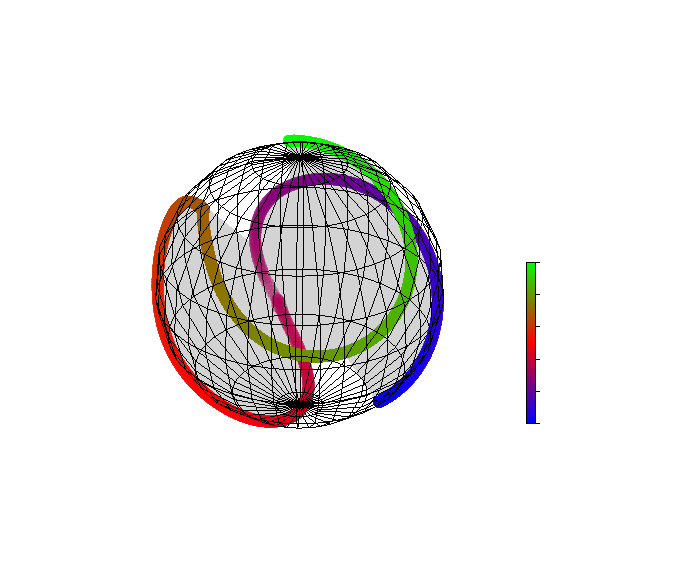
\includegraphics[width=0.55\linewidth]{chapters/ch-experiments/img/tc.pdf}
    % }
    \subfigure[`\textit{pour milk}' from activity ``\textit{cereal}'']{\label{subfig:pmc}
    \begin{overpic}[width=0.47\linewidth]{chapters/ch-experiments/img/tc.pdf}
        \put(93,3){\footnotesize 0.0}
        \put(93,9.5){\footnotesize 0.2}
        \put(93,16){\footnotesize 0.4}
        \put(93,22.5){\footnotesize 0.6}
        \put(93,29){\footnotesize 0.8}
        \put(92.9,35.5){\footnotesize 1.0}
        \put(80,5.5){ $c\!:$}
    \end{overpic}
    }\\
    \hfill
    \subfigure[`\textit{pour milk}' from activity ``\textit{cereal}'']{\label{subfig:pmc2}
    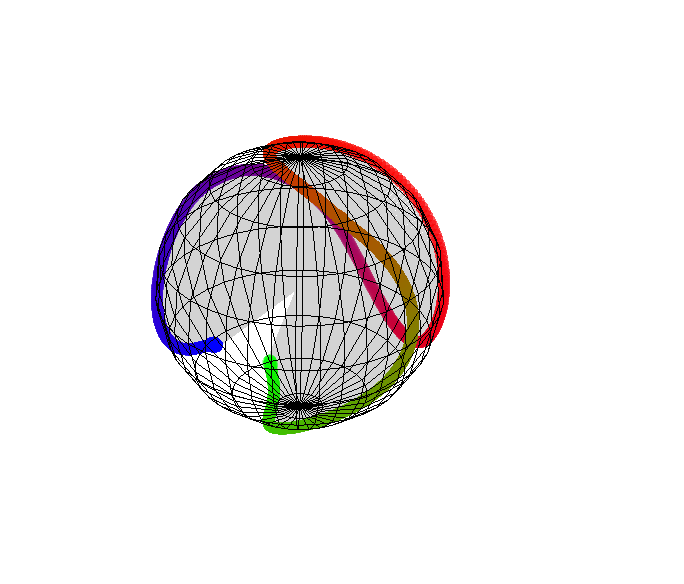
\includegraphics[width=0.33\linewidth]{chapters/ch-experiments/tex/pour_milk_cereal_2.pdf}
    }\hfill
    \subfigure[`\textit{take knife}' from activity ``\textit{juice}'']{\label{subfig:tkj}
    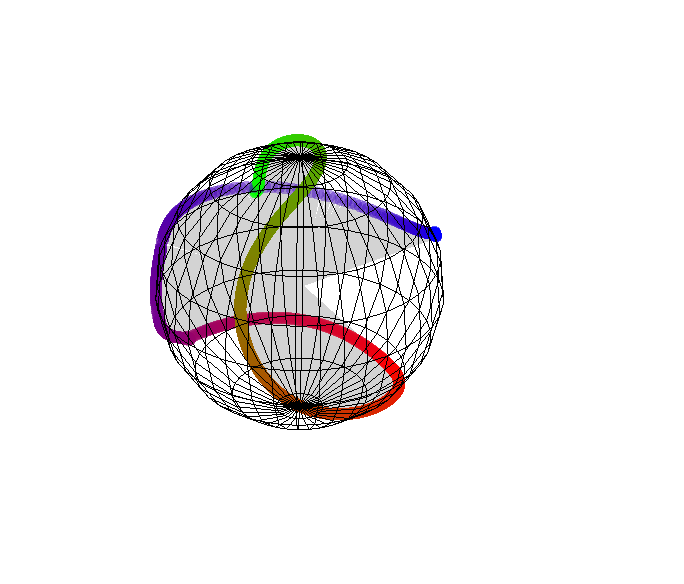
\includegraphics[width=0.33\linewidth]{chapters/ch-experiments/img/take_knife_juice.pdf}
    }\hfill
    \caption{T-SNE visualizations of generated action segments. %Every point in the sphere corresponds to a frame feature, and the continuity of these feature points demonstrates temporal coherence.
    }\label{fig:viz}
\end{figure}

To assess the temporal coherence of the generated samples, we employ T-SNE~\cite{van2008visualizing} to visualize action segments generated by our TCA model. Every point in the sphere corresponds to a frame feature. Each segment comprises 1,000 frames, each sharing a common action label $a$ and latent variable $z$, with an evenly strided $c$. 

Specifically, we employ the TCA model trained on ``\textit{cereal}'' data to generate an action segment of `\textit{pour milk}' in~\cref{subfig:pmc}. \cref{subfig:pmc2} depicts the same action of `\textit{pour milk}' for ``\textit{cereal}'' but is generated using a different latent variable $z$, highlighting the diversity in trajectories. \cref{subfig:tkj} shows a generated segment of a different action `\textit{take knife}' from ``\textit{juice}''. All visualized action segments exhibit continuous properties in the feature space, corresponding to the gradual increase in the coherence variable $c$, showcasing the temporal coherence between the frame features.